\chapter{Introduction}\label{introduction}

\section{Background and Motivation}

The CESAR project aim to use low cost sensor kit to prototype applications using physiological signals related to heart rate, brain activity, oxygen level in blood to monitor sleep and breathing related illnesses, like Obstructive Sleep Apnea (OSA). Side effects of OSA do not only cause sleepiness during day time (which might affect daily chores), but also serious illnesses like diabetes and cardiac dysfunctions. Statistically speaking, it is estimated that about 25\% of the adult population in Norway has OSA, but only 10\% of them are diagnosed. A major problem with diagnosing OSA is polysomnography in \textit{sleep laboratories} \cite{cesar}. This is both really expensive and inefficient due to lacking capacity to perform sufficient tests with patients. Hence, the CESAR project aims to contribute to this situation with a low-cost Android and BiTalino based system to tackle these problems in a minimal invasive approach. 

The project has been developed by various people over the years, and the system has been divided into three parts (illustrated in Figure \ref{fig:parts}). The data acquisition part, the data streams dispatching part, and the application part. The first two parts are already implemented (summarized in the section below), thus, the last part is what we will be focusing throughout this thesis. 

\begin{figure}
    \centering
    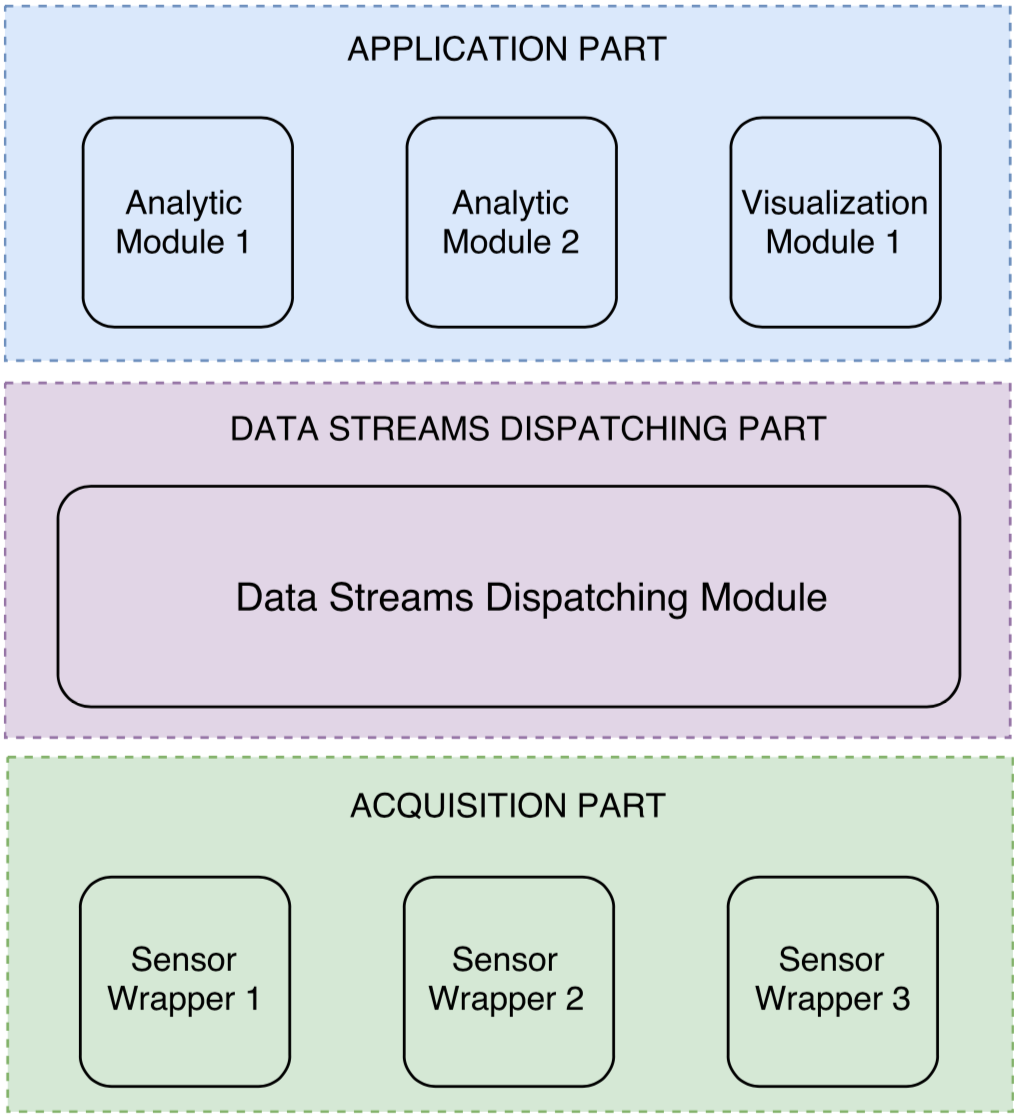
\includegraphics[width=0.5\textwidth]{images/parts.png}
    \caption{Structure of the project, separating functionality into three independent layers \cite{daniel}}
    \label{fig:parts}
\end{figure}

\section{Problem Statement}

The market has new and affordable sensors that can aid with the data acquisition, which we seamlessly can integrate with the extensible data streams dispatching tool. The Flow sensor is an interesting sensor source due to its versatility and adaptability of collecting breathing data and connecting to devices with the BlueTooth protocol. 

As for the state of this thesis: (i) applications which supports the Flow sensor has not been designed for end-users, in essence, they provide no user-friendly interface that allows for sharing of the data. In order to extract the data from these applications, the mobile device has to be connected with a PC over USB for data transfer; (ii) there is no sensor wrappers that support the Flow sensor with the data streams dispatching tool in the CESAR project; and (iii) the data streams dispatching tool is not ready to be used by the end-users, because the project facilitates no user-friendly interface for users to record the data from the supported sensor sources.

As such, we look into designing and implementing an Android application (Nidra) that record, share, and analyze breathing data over an extended period (e.g., during sleep) by using the Flow sensor. Additionally, we want to facilitate an extensible application such that future developers can extend functionality or enrich the data in Nidra. In the end, we can hopefully strengthen the analysis of abnormal sleeping patterns to decreasing the risk of the symptoms they may come as a consequence. Also, as a bi-product, the application can be used in other fields of studies (e.g., physical activities). As the scope of this thesis, we focus on the completion of three main goals:

\begin{description}
    \item[Goal 1] Integrate the support for Flow sensor by creating a sensor wrapper that connects with the extensible data streams dispatching tool.
    \item[Goal 2] Research and develop a user-friendly application which facilitates collection of breathing data with the Flow sensor, sharing of the data, and analysis of the data with the use of the extensible data streams dispatching tool.
    \item[Goal 3] Create an extensible solution such that the developers can create standalone applications that integrate with Nidra. 
\end{description}

As part of the goals of this thesis, we also define three system requirements to keep in mind while designing and implementing the application. The three system requirements are the following: 

\begin{description}
    \item[Requirement 1] The application must provide an interface for the patient to (i) record physiological signals (e.g., breathing data); (ii) present the results; and (iii) share the results.
    \item[Requirement 2] The application must ensure that upon sensor disconnections, the connectivity is reinstated to minimize the data loss and its effects on the data analysis.
    \item[Requirement 3] The application must provide an interface for the developers to create modules that integrate with the application.
\end{description}



\section{Limitations}
Based on the objectives and requirements defined in the previous section, the scope of this thesis is to design and implement an application capable of recording physiological obtained by the Flow sensor kit over an extended period. 

We limited the scope of testing for existing sensor source development, and the support for future sensor sources. Further, with the Flow sensor kit provided under development, we restricted the design to collect respiration (breathing) data (opposed to hearthrate).

Additionally, the implementation is Android specific as the previous work performed on the project is designed soley for Android applications. 

\section{Research Methods}
The work in this thesis can be classified as \textit{computing research} with a principle approach of an \textit{engineering method} as described in [cite]. The engineering method (evolutionary paradigm) is to: (i) observe existing methods, (ii) propose better solution, (iii)  build or develop artifacts\footnote{human-manufactured objects produced during the development}, and (iv) measure and analyze until no further improvements are possible [CITE]. The report identifies patterns amongst various principle approaches and categorizes the the pattern into phases: \textit{(i) informational phase}, \textit{(ii) propositional phase}, \textit{(iii) analytical phase}, and \textit{(iv) evaluation phase}. Below, we give a brief description of each phase and discuss how our work fits into each of them. 

\subsection{Informational Phase}
The informational phase according to the report is to \textit{"gather or aggregate information via reflection, literature survey, people/organization survey, or poll"}

As part of this thesis is to design and implement an application that collects respiration data during sleep, and to future analyze and examinate the respration data to detect sleep related-breathing disorders (e.g., Obstructive Sleep Apnea), we conducted a survey on previous related work in Chapther 3.

\subsection{Propositional Phase}
The propositional phase according to the report is to \textit{"propose and/or formulate a hypothesis, method or algorithm, model, theory, or solution"}

Based on the related work, one of the goals of this thesis is to create an extensible application that allows future "related" applications to extend the functionality or enrich the data in our application. Also, to create an application which will be used to record, share and analyze respiration data collected over an extended period. 

\subsection{Analytical Phase}
The analytical phase according to the report is to \textit{"analyze and explore a proposition, leading to a demonstration and/or formulation of a principle or theory"}

In the design chapther of this thesis, we analyze and explore various methods of implementing a functionality/task. In the implementation chapther of this thesis, we demonstrate the design choices by developing an Android application which follows the design. 

\subsection{Evaluation Phase}
The evaluation phase according to the report is to \textit{"evaluate a proposition or analytic finding by means of experimentation (controlled) or observation (uncontrolled, such as a case study or protocol analysis), perhaps leading to a substantiated model, principle, or theory"}

Based on the requirements and goal of this thesis, we performed various experiements to evaluate the performance of the application.

\section{Contributions}
Over the course of this thesis, we design and implemented an application for collecting, sharing and analyzing breathing data and a platform for modules to enrich the applications, called Nidra. The application is focused on creating a generalized application which manges sensor data with focus on sleep apnea / collecting data during sleep over an extended period, which purpose was to enable analyzing and sharing of the data with researchers/doctors.  

Through the work produced in this thesis, 


\section{Thesis Outline}
The thesis is divided into three parts, which the following list presents a general overview of:

\begin{itemize}
    \item Part 1: \textbf{Introduction \& Background}
    \begin{description}[font=\normalfont\itshape]
        \item[Chapther 2: Background] presents the background material necessary for understanding the fundamentals in this thesis. It starts by introducing the CESAR project and the tools provided for data acquisition. Then, an overview of the Android operating system architecture and components are 
        \item[Chapther 3: Related Work] presents the related work focusing on creating a mobile applicaton to collect physiological data in order to diagnose sleep apnea. Finally, we discuss why our solution is an improvement to the related work.
    \end{description}

    \item Part 2: \textbf{Design \& Implementation}
    \begin{description}[font=\normalfont\itshape]
        \item[Chapther 4: Analysis and High-Level Design] encompasses the functional requirements, the design purposal, and the structure of the data in the application.
        \item[Chapther 5: Implementation] realizes the design purposal in Android, with the use of the previous work.
    \end{description}

    \item Part 3: \textbf{Evaluation \& Conclusion}
    
    \begin{description}[font=\normalfont\itshape]
        \item[Chapther 6: Evaluation] conducts various experiements in order to tests if the system requirements is fullfilling.
        \item[Chapther 7: Conclusion] discuss the objectives and the overall goal of the thesis, with suggestions to future work.
    \end{description}

\end{itemize}

